\section{Optimizing matrix multiplication on GPUs}%
\label{sec:matmul}

Matrix multiplication is a common mathematical function, which has many applications.
In this project matrix multiplication can be used in fully connected layers and in a convolutional layers.
The optimizations that will be discussed in this section is only discussed for how it could be done.
Since this project relies on Futhark, these optimizations have not been implemented in the library.

Since GPUs are massively parallel and matrix multiplication can be made highly parallel, it makes sense to use GPUs for matrix multiplication of large data quantities.
Even though matrix multiplication can be quite simple to implement, it is not trivial to implement an effecient matrix multiplication implementation for GPUs.
The problem is that GPUs does not have that much space for caching, also fetching data from global memory in the GPU can be very slow, compared to using data from shared memory.
Matrix multiplication reuses the same data many times, in fact $O(n)$ data reuses \cite{performant_gemm}.
This data reuse is the part that should be treated carefully since it is far better to use the data from shared memory.

% Consider ineffecient example?

The general idea for GEMM is to use tiles from the input matrices.
The tiles should be chosen such that they fit into the available fast or shared memory.
As computations of different tiles of the resultant
matrix are independent, those can be performed completely
in parallel to maximise the resource utilisation of massively
parallel GPUs \cite{performant_gemm}.
\autoref{fig:gemm} shows how a tile from two matrices $A$ and $B$ can be multiplied together in $C$.
\begin{figure}
  \centering
  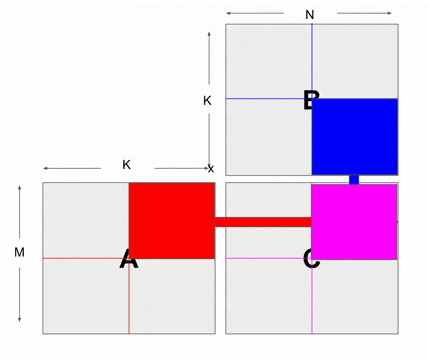
\includegraphics[width=0.45\textwidth]{assets/gemm.png}
  \caption{A visual representation of how to tiles in $A$ and $B$ might be added together in $C$. Source: \cite{gemm}}
  \label{fig:gemm}
\end{figure}
Each time two tiles are multiplied, the result is stored in the tile in $C$, however if this has to happen in parallel it cannot just add the result to the $C$ matrix.
Instead an array for each entry in $C$ can be created and then summed up later, this exploits even more parallelism while still keeping the tiles so that it can access the memory quickly.
